\documentclass[12pt]{article}
\usepackage{listings}
\usepackage{color}
\usepackage{enumitem}
\usepackage{amsmath}
\usepackage{hyperref}
\usepackage{pgfplots}
\usepackage{circuitikz}
\usepackage{graphicx}
\usepackage{subcaption}
\usepackage[utf8]{inputenc}
\usepackage{siunitx}
\usepackage{multirow}

\usetikzlibrary{positioning}

\definecolor{dkgreen}{rgb}{0,0.6,0}
\definecolor{gray}{rgb}{0.5,0.5,0.5}
\definecolor{mauve}{rgb}{0.58,0,0.82}

\lstset{frame=tb,
  language=Bash,
  aboveskip=3mm,
  belowskip=3mm,
  showstringspaces=false,
  columns=flexible,
  basicstyle={\small\ttfamily},
  breaklines=true,
  breakatwhitespace=true,
  tabsize=3
}
\sisetup{
  round-mode          = places,
  round-precision     = 2, 
}

\author{Micha\l{} Tracewicz}
\date{2020-03-07}
\title{\LaTeX - Introduction}
\begin{document}
\pagenumbering{gobble}
\maketitle
\newpage
\tableofcontents
\newpage
\pagenumbering{arabic}
\section{What is \LaTeX?}
\LaTeX is a markup language to typeset documents.
It can be understood as a way to programmatically create documents.
\section{Compiling document}
Document written using \LaTeX need to be compiled before they are rendered into output file.
First of user needs to install \LaTeX. In Ubuntu Linux this can be done with following commands:
\begin{lstlisting}
    sudo apt install textlive
    sudo apt-get install texlive-latex-extra
    sudo apt-get install texlive-science
\end{lstlisting}
User should create '.tex' file in which they write their document using \LaTeX.
Afterwards this document should be compiled using following command:
\begin{lstlisting}
    pdflatex [source file path]
\end{lstlisting}
It will produce '.pdf' file in current directory.
\section{Document structure}
\subsection{Basic document structure}
\LaTeX uses commands to do format, structuring document etc.
For example:
\begin{verbatim}
    \section{Name}
\end{verbatim}
This will create numbered section in document with heading "Name".
Basic \LaTeX document should look something like this:
\begin{verbatim}
\documentclass{article}
\begin{document}
  Hello World!
\end{document}
\end{verbatim}
It begins with with:
\begin{verbatim}
\documentclass{article}
\end{verbatim}
All of \LaTeX commands starts with '\textbackslash'.
First line of our document should be documentclass command.
It determines how the whole document will be rendered. "article" is one of most common classes. Other notable
options are "book", "report", "slides", "beamer" (the last one is used to create presentations).
Next we have:
\begin{verbatim}
\begin{document}
    Hello World!
\end{document}
\end{verbatim}
Here we create an environment. It is possible to create multiple environments in one document.
They are parts of document to which certain typesetting rules apply.
Inside it author inserts content of theirs document.
Everything which will be put between those two segments is called a "Preamble".
Here user can point which packages will be used (more on this later), insert metadata from which
document title page will be created. Things which are in preamble will not be directly rendered on document.
For example lets take a look at part of this documents preamble:
\begin{verbatim}
\documentclass[12pt]{article}
\usepackage{listings}

\author{Michał Tracewicz}
\date{2020-03-07}
\title{\LaTeX - Introduction}

\begin{document}
\pagenumbering{gobble}
\maketitle
\newpage
\pagenumbering{arabic}
\end{document}
\end{verbatim}
Document title, author and date are inserted and then later on rendered with:
\begin{verbatim}
    \maketitle
\end{verbatim}
Looking at this snippet there are some more interesting commands
\begin{verbatim}
    \pagenumbering{gobble}
    \newpage
    \pagenumbering{arabic}
\end{verbatim}
Going top to bottom first user disables title page from being numbered. Then user forces new page to make sure 
only title is placed on first page. Next command enables numbering of pages using arabic numbers.
To force \LaTeX to create new line use "\textbackslash\textbackslash",
to force new line use "\textbackslash newline", new page "\textbackslash newpage"
\subsection{Sections, paragraphs}
\LaTeX gives its users a way to automaticly create and number section headings.
In addition user can create headings without numbering using paragraphs.
To structure document one can use those commands:
\begin{verbatim}
    \section{Section name}
    \subsection{Subsection name}
    \subsubsection{Subsubsection name}

    \paragraph{Paragraph name}
    \subparagraph{Subparagraph name}
\end{verbatim}
\subsection{Packages}
\LaTeX has a lot of both user created and built in packages.
To find packages visit: \href{https://www.ctan.org/pkg}{ctan.org}
User can download and remove packages by using:
\begin{lstlisting}
tlmgr install <package1> <package2> ...
tlmgr remove <package1> <package2> ...
\end{lstlisting}
To use package we need to register it using
\begin{verbatim}
\usepackage{listings}
\end{verbatim}
Doing so will give user ability to use commands provided in package.
This particular package provides way to do source code highlighting.
It will be described in later section.
\subsection{Table of contents}
If user had used sections to structure theirs document \LaTeX provides a command to create table of contents
based sections, subsections,subsubsections.
\begin{verbatim}
    \tableofcontents
\end{verbatim}
\subsection{Lists}
When writing \LaTeX documents user has an ability to create both ordered and unordered lists.
\subsubsection{Unordered lists}
Following snippet can be used to create unordered list which will contain three entries named
"First", "Second", "Third":
\begin{verbatim}
    \begin{itemize}
        \item First
        \item Second
        \item Third
    \end{itemize}
\end{verbatim}
This wil render as:
\begin{itemize}
    \item First
    \item Second
    \item Third
\end{itemize}
When working with unordered lists sometimes it is desireable to change item symbol.
This can be done by:
\begin{verbatim}
    \begin{itemize}
        \item[--] Dash
        \item[$\ast$] Asterisk
        \item[$\beta$] Any mathematical symbol
    \end{itemize}
\end{verbatim}
Which will render as:
\begin{itemize}
    \item[--] Dash
    \item[$\ast$] Asterisk
    \item[$\beta$] Any mathematical symbol
\end{itemize}
To change symbol for all elements we will use package and it will be 
demonstrated in Ordered List section.
\subsubsection{Ordered lists}
Following snippet can be used to create ordered list which will contain three entries named
"First", "Second", "Third":
\begin{verbatim}
    \begin{enumerate}
        \item First
        \item Second
        \item Third
    \end{enumerate}
\end{verbatim}
This will render as:
\begin{enumerate}
    \item First
    \item Second
    \item Third
\end{enumerate}
Changing enumeration can be done in two steps.
First user needs to add this to theirs preamble:
\begin{verbatim}
    \usepackage{enumitem}
\end{verbatim}
Then we can use following:
\begin{verbatim}
% Roman numbers
\begin{enumerate}[label=(\roman*)]
    \item First
    \item Second
    \item Third
\end{enumerate}

% Arabic numbers
\begin{enumerate}[label=\arabic*)]
    \item First
    \item Second
    \item Third
\end{enumerate}

% Alphabetical
\begin{enumerate}[label=\alph*)]
    \item First
    \item Second
    \item Third
\end{enumerate}
\end{verbatim}
Which will render as:
\begin{enumerate}[label=(\roman*)]
    \item First
    \item Second
    \item Third
\end{enumerate}
\begin{enumerate}[label=\arabic*)]
    \item First
    \item Second
    \item Third
\end{enumerate}
\begin{enumerate}[label=\alph*)]
    \item First
    \item Second
    \item Third
\end{enumerate}
This can also be used to change symbols in unordered lists:
\begin{verbatim}
    \begin{itemize}[label=$\ast$)]
        \item First
        \item Second
        \item Third
    \end{itemize}
\end{verbatim}
Which will render as:
\begin{itemize}[label=$\ast$)]
    \item First
    \item Second
    \item Third
\end{itemize}
\subsubsection{Nested lists}
Following snippet can be used to create nested ordered list which will contain five entries named
"First" - it will contain subentries "Second" and "Third", "Fourth", "Fifth"
\begin{verbatim}
    \begin{enumerate}
        \item First
        \begin{enumerate}
            \item Second
            \item Third
        \end{enumerate}
        \item Fourth
        \item Fifth
    \end{enumerate}
\end{verbatim}
This will render as:
\begin{enumerate}
    \item First
    \begin{enumerate}
        \item Second
        \item Third
    \end{enumerate}
    \item Fourth
    \item Fifth
\end{enumerate}
\subsection{Footnotes}
In \LaTeX there are is an easy way of creating and referring footnotes.
\begin{verbatim}
    Example \footnote{\label{myfootnote} Hello footnote}
    Referring to footnote \ref{myfootnote}
\end{verbatim}
Which will render as:
Example \footnote{\label{myfootnote} Hello footnote}
Referring to footnote\ref{myfootnote}
Footnotes are numbered automatically.
It is imperative, that the label is contained in footnote,
otherwise the label will refer to section
\section{Mathematics}
\LaTeX is designed in a way which makes it easy to insert mathematical equations.
There are two options how user can handle inputting maths into document.
The first one is embedding the formula inline directly into the text.
This can be done using \$.
For example:
\begin{verbatim}
    Exponential functions can look like this: $f(x) = 2^x$
\end{verbatim}
Which will render as:
Exponential functions can look like this: $f(x) = 2^x$
Second option includes creating new environment.
Two main math environments are "equation" which is used to render one equation 
(if user try's to enter more it will result in compilation error)
and "align" which is used to render multiple equations at the same time.
Examples:
\begin{verbatim}
    \usepackage{amsmath}
    % Code omitted for clarity...
    \begin{equation*}
        f(x) = \frac{1}{x}
    \end{equation*}
    \begin{align*}
        1 + 2x &= 3 \\
            3x &= 5 - 2
    \end{align*}
\end{verbatim}
This will be rendered as:
\begin{equation*}
    f(x) = \frac{1}{x}
\end{equation*}
\begin{align*}
    1 + 2x &= 3 \\
        3x &= 5 - 2
\end{align*}
Lets take a closer look at "align" environment.
As its name suggests, it will align equations. This will happen at '\&' sign.
Each equation needs to be separated with "\textbackslash\textbackslash".
Asterisk at the end of both environments are used to indicate that user doesn't want them to be numbered.
\LaTeX is capable of displaying much more complicated equations some notable examples:
\begin{verbatim}
\begin{align*}
\left[
\begin{matrix}
1 & 0\\
0 & 1
\end{matrix}
\right]
&\ast
\left[
\begin{matrix}
a & b\\
c & d
\end{matrix}
\right]
=
\left[
\begin{matrix}
a & b\\
c & d
\end{matrix}
\right]\\
&\int^b_a\left(\frac{1}{\sqrt{x\pi}}\right)\\
T^{i_1 i_2 \dots i_p}_{j_1 j_2 \dots j_q} &= (line broken for clarity)
T(x^{i_1},\dots,x^{i_p},e_{j_1},\dots,e_{j_q})
\end{align*}
\end{verbatim}
Which is rendered as:
\begin{align*}
\left[
\begin{matrix}
1 & 0\\
0 & 1
\end{matrix}
\right]
&\ast
\left[
\begin{matrix}
a & b\\
c & d
\end{matrix}
\right]
=
\left[
\begin{matrix}
a & b\\
c & d
\end{matrix}
\right]\\
&\int^b_a\left(\frac{1}{\sqrt{x\pi}}\right)\\
T^{i_1 i_2 \dots i_p}_{j_1 j_2 \dots j_q} &= T(x^{i_1},\dots,x^{i_p},e_{j_1},\dots,e_{j_q})\\
\lim^{}_{x->\inf}\frac{1}{x} &= 0
\end{align*}
Lets take a closer look. To create matrix user creates
\begin{verbatim}
\left[
\begin{matrix}
a & b\\
c & d
\end{matrix}
\right]
\end{verbatim}
\textbackslash left[ and \textbackslash right] are responsible for creation of scaling braces around matrix.
Then it is created using "matrix" environment, 
new line character ("\textbackslash\textbackslash") is responsible for creating new row.
\textbackslash int - integral symbol\\
\textbackslash frac - fractions\\
\textbackslash sqrt - square root\\
"\textasciicircum\{a\}\_\{b\}" - is used to create indexes where "a" is top and "b" is bottom)\\
\textbackslash dots - inserts "..."\\
\textbackslash pi - inserts Pi symbol (any greek letter can be inserted in the same fashion)\\
\section{Pictures}
A lot of documents need pictures to present their content properly. \LaTeX allow users to
insert images by using this package "graphicx".
Lets insert first image:
\begin{verbatim}
\begin{figure}[h!]
    \centering
    \begin{subfigure}[b]{0.4\linewidth}
        
\includegraphics[width=\linewidth]{coffee.jpg}
        \caption{Coffee.}
    \end{subfigure}
    \label{fig:coffee}
\end{figure}
\end{verbatim}
Which will be rendered as:
\begin{figure}[h!]
    \centering
    \begin{subfigure}[b]{0.4\linewidth}
      
\includegraphics[width=\linewidth]{coffee.jpg}
      \caption{Coffee.}
    \end{subfigure}
    \caption{Coffee picture}
    \label{fig:coffee}
\end{figure}
Figure environment will take care of numbering and positioning of image. To include image user needs to
use \textbackslash includegraphics and pass a path to picture in curly braces. In this example width is set top
0.4\textbackslash linewidth which means that picture will be scaled up/down to take 0.4 of document width.
\textbackslash caption allows user to add visible caption to an image, \textbackslash label adds invisible label
which can be helpful if user wants to refer to this image later on.
User can suggest or force how \LaTeX will position an image. It is done by putting one of following values into squere
brackets after \textbackslash begin{figure}:
\begin{itemize}
    \item h (here) - same location
    \item t (top) - top of page
    \item b (bottom) - bottom of page
    \item p (page) - on an extra page
    \item ! (override) - will force the specified location
\end{itemize}
Sometimes there is the need to compare two images thankfully \LaTeX
allows to do this pretty easily by using "subcaption" package.
\begin{verbatim}
\begin{figure}[h!]
    \centering
    \begin{subfigure}[b]{0.4\linewidth}
        
\includegraphics[width=\linewidth]{coffee.jpg}
        \caption{Coffee.}
        \label{fig:coffee1}
    \end{subfigure}
    \begin{subfigure}[b]{0.4\linewidth}
        
\includegraphics[width=\linewidth]{coffee.jpg}
        \caption{another Coffee.}
        \label{fig:coffee2}
    \end{subfigure}
    \caption{Coffee comparison.}
    \label{fig:coffecomparison}
\end{figure}
\end{verbatim}
Which renders as:
\begin{figure}[h!]
    \centering
    \begin{subfigure}[b]{0.4\linewidth}
      
\includegraphics[width=\linewidth]{coffee.jpg}
      \caption{Coffee.}
      \label{fig:coffee1}
    \end{subfigure}
    \begin{subfigure}[b]{0.4\linewidth}
        
\includegraphics[width=\linewidth]{coffee.jpg}
        \caption{another Coffee.}
        \label{fig:coffee2}
    \end{subfigure}
    \caption{Coffee comparison.}
    \label{fig:coffecomparison}
\end{figure}
\section{Bibliography}
To automate creation of bibliography user needs to use external tools like:
"Bibtex" or "Biblatex". To use BibTex we simply need to add :
\begin{verbatim}
\bibliography{bibliography_file}
\bibliographystyle{ieeetr}
\end{verbatim}
just before \textbackslash end{document}.
First command is used to tell BibTex which file ".bib" file should it use and second one is
responsible for setting style in which our bibliography will be displayed. ".bib" files can easily be created
with online editors. To use citation in our document we need to insert
\begin{verbatim}
    \cite{WEBSITE:1}
\end{verbatim} \cite{WEBSITE:1} as I did here. Most of the examples I used in this article are come from
this site, some others come from \cite{WEBSITE:2} and the rest are either from \cite{WEBSITE:3}.
Coffee image was taken from \cite{IMAGE:1}.
If we add BibTex we need to change our compilation process to:
\begin{lstlisting}
    pdflatex [source file path]
    bibtex [source file path]
    pdflatex [source file path]
    pdflatex [source file path]
\end{lstlisting}
as presented in\cite{WEBSITE:4}, reader can also find how to use Biblatex in the same article.
\section{Tables}
To create tables user needs to combine two environments, "table" and "tabular".
Example code to create table looks like this:\\
\begin{verbatim}
\begin{table}[h!]
\begin{center}
    \caption{Your first table.}
    \label{tab:table1}
    \begin{tabular}{l|c|r}
    \textbf{Value 1} & \textbf{Value 2} & \textbf{Value 3}\\
    $\alpha$ & $\beta$ & $\gamma$ \\
    \hline
    1 & 1110.1 & a\\
    2 & 10.1 & b\\
    3 & 23.113231 & c\\
    \end{tabular}
\end{center}
\end{table}
\end{verbatim}
Which will render as:
\begin{table}[h!]
\begin{center}
    \caption{Your first table.}
    \label{tab:table1}
    \begin{tabular}{l|c|r}
    \textbf{Value 1} & \textbf{Value 2} & \textbf{Value 3}\\
    $\alpha$ & $\beta$ & $\gamma$ \\
    \hline
    1 & 1110.1 & a\\
    2 & 10.1 & b\\
    3 & 23.113231 & c\\
    \end{tabular}
\end{center}
\end{table}
"table" environment is responsible for holding tables caption, label and its positioning on page.
It works in the same way as with \ref{fig:coffee} on page~\pageref{fig:coffee}.
"tabular" environment is used to create table itself. "\&" is used as column separator and "\textbackslash\textbackslash"
is used as new row. Vertical lines are passed in square brackets to "tabular" environment as "|" character.
The letters which are next to them tell \LaTeX how to align content in column:
\begin{itemize}
    \item l - left
    \item c - center
    \item r - right
\end{itemize}
Row separators can be added with \textbackslash hline. To align numbers according to decimal point use
needs to include "siunitx" package and configure it. Example configuration looks something like this:
\begin{verbatim}
\usepackage{siunitx} 
\sisetup{
  round-mode          = places,
  round-precision     = 2,
}
\end{verbatim}
Now when this is done user can use new option when setting column alignment "S".
For example:
\begin{table}[h!]
\begin{center}
    \caption{Your second table.}
    \label{tab:table2}
    \begin{tabular}{l|S|r}
    \textbf{Value 1} & \textbf{Value 2} & \textbf{Value 3}\\
    $\alpha$ & $\beta$ & $\gamma$ \\
    \hline
    1 & 1110.1 & a\\
    2 & 10.1 & b\\
    3 & 23.113231 & c\\
    \end{tabular}
\end{center}
\end{table}
Sometimes it is necessary for a cell to span multiple rows and/or columns.
This can be done with "multirow"and "multicolumn" commands.
To use them we need to include "mutirow" package.
lets start with multirow. It takes three arguments: NUMBER\_OF\_ROWS, WIDTH, CONTENT.
Width can be set to "*" to make it automatic.
Example presenting alpha value spanning two rows:
\begin{verbatim}
\begin{table}[h!]
\begin{center}
    \caption{Multirow table.}
    \label{tab:table3}
    \begin{tabular}{l|S|r}
    \textbf{Value 1} & \textbf{Value 2} & \textbf{Value 3}\\
    $\alpha$ & $\beta$ & $\gamma$ \\
    \hline
    \multirow{2}{*}{12} & 1110.1 & a\\
    & 10.1 & b\\
    \hline
    3 & 23.113231 & c\\
    4 & 25.113231 & d\\
    \end{tabular}
\end{center}
\end{table}
\end{verbatim}
\begin{table}[h!]
\begin{center}
    \caption{Multirow table.}
    \label{tab:table3}
    \begin{tabular}{l|S|r}
    \textbf{Value 1} & \textbf{Value 2} & \textbf{Value 3}\\
    $\alpha$ & $\beta$ & $\gamma$ \\
    \hline
    \multirow{2}{*}{12} & 1110.1 & a\\
    & 10.1 & b\\
    \hline
    3 & 23.113231 & c\\
    4 & 25.113231 & d\\
    \end{tabular}
\end{center}
\end{table}
Multicolumn command has the same number of arguments and they are: NUMBER\_OF\_COLUMNS, ALIGNMENT, CONTENT.
\begin{verbatim}
\begin{table}[h!]
\begin{center}
    \caption{Multicolumn table.}
    \label{tab:table4}
    \begin{tabular}{l|S|r}
    \textbf{Value 1} & \textbf{Value 2} & \textbf{Value 3}\\
    $\alpha$ & $\beta$ & $\gamma$ \\
    \hline
    \multicolumn{2}{c|}{12} & a\\
    \hline
    2 & 10.1 & b\\
    3 & 23.113231 & c\\
    4 & 25.113231 & d\\
    \end{tabular}
\end{center}
\end{table}
\end{verbatim}
Which will render as:
\begin{table}[h!]
\begin{center}
    \caption{Multicolumn table.}
    \label{tab:table4}
    \begin{tabular}{l|S|r}
    \textbf{Value 1} & \textbf{Value 2} & \textbf{Value 3}\\
    $\alpha$ & $\beta$ & $\gamma$ \\
    \hline
    \multicolumn{2}{c|}{12} & a\\
    \hline
    2 & 10.1 & b\\
    3 & 23.113231 & c\\
    4 & 25.113231 & d\\
    \end{tabular}
\end{center}
\end{table}
Those two commands can be combined like this:
\begin{verbatim}
\begin{table}[h!]
\begin{center}
    \caption{Multirow and -column table.}
    \label{tab:table5}
    \begin{tabular}{l|S|r}
    \textbf{Value 1} & \textbf{Value 2} & \textbf{Value 3}\\
    $\alpha$ & $\beta$ & $\gamma$ \\
    \hline
    \multicolumn{2}{c|}{\multirow{2}{*}{1234}} & a\\
    \multicolumn{2}{c|}{} & b\\ 
    \hline
    3 & 23.113231 & c\\
    4 & 25.113231 & d\\
    \end{tabular}
\end{center}
\end{table}
\end{verbatim}
Which will look like:
\begin{table}[h!]
\begin{center}
    \caption{Multirow and -column table.}
    \label{tab:table5}
    \begin{tabular}{l|S|r}
    \textbf{Value 1} & \textbf{Value 2} & \textbf{Value 3}\\
    $\alpha$ & $\beta$ & $\gamma$ \\
    \hline
    \multicolumn{2}{c|}{\multirow{2}{*}{1234}} & a\\
    \multicolumn{2}{c|}{} & b\\
    \hline
    3 & 23.113231 & c\\
    4 & 25.113231 & d\\
    \end{tabular}
\end{center}
\end{table}
\LaTeX provides a way of inserting tables which are multiple pages long ("longtable" environment),
in landscape mode ("sidewaystable" environment from "rotating" package) and even loading them
from ".csv" ("pgfplotstable" package) however this is beyond the scope of this article.
\section{Source code}
When writing about programing it is necessary to include code snippets in document.
To do this in \LaTeX we need to first include two packages:
\begin{verbatim}
\usepackage{listings}
\usepackage{color}
\end{verbatim}
next step is to configure syntax highlighting:
\begin{verbatim}
\definecolor{dkgreen}{rgb}{0,0.6,0}
\definecolor{gray}{rgb}{0.5,0.5,0.5}
\definecolor{mauve}{rgb}{0.58,0,0.82}

% This will be configured for all listings in document
\lstset{frame=tb,
    language=Python,
    aboveskip=3mm,
    belowskip=3mm,
    showstringspaces=false,
    columns=flexible,
    basicstyle={\small\ttfamily},
    numbers=none,
    numberstyle=\tiny\color{gray},
    keywordstyle=\color{blue},
    commentstyle=\color{dkgreen},
    stringstyle=\color{mauve},
    breaklines=true,
    breakatwhitespace=true,
    tabsize=3
}
\end{verbatim}
Above example sets up syntax highlighting for Python.
Afterwards we can insert code by creating new environments:
\begin{verbatim}
% Here in "[]" user configures settings only for current listing
\begin{lstlisting}[frame=tb,
    language=Python,
    aboveskip=3mm,
    belowskip=3mm,
    showstringspaces=false,
    columns=flexible,
    basicstyle={\small\ttfamily},
    numbers=none,
    numberstyle=\tiny\color{gray},
    keywordstyle=\color{blue},
    commentstyle=\color{dkgreen},
    stringstyle=\color{mauve},
    breaklines=true,
    breakatwhitespace=true,
    tabsize=3]
import numpy as np
a = np.arange(0,60,5)
a = a.reshape(3,4)

print(f'Original array is:\n{a}')
print(f'Transpose of the original array is:\n{a.T}')
\end{lstlisting}
\end{verbatim}
Which will be rendered as:
\begin{lstlisting}[frame=tb,
    language=Python,
    aboveskip=3mm,
    belowskip=3mm,
    showstringspaces=false,
    columns=flexible,
    basicstyle={\small\ttfamily},
    numbers=none,
    numberstyle=\tiny\color{gray},
    keywordstyle=\color{blue},
    commentstyle=\color{dkgreen},
    stringstyle=\color{mauve},
    breaklines=true,
    breakatwhitespace=true,
    tabsize=3]
import numpy as np
a = np.arange(0,60,5)
a = a.reshape(3,4)

print(f'Original array is:\n{a}')
print(f'Transpose of the original array is:\n{a.T}')
\end{lstlisting}
\section{Drawing}
In \LaTeX it is possible to plot functions and draw, to do so user needs to include package "pgfplots".
Package documentations: \href{https://mirrors.nic.cz/tex-archive/graphics/pgf/contrib/pgfplots/doc/pgfplots.pdf}{Pdfplots}
Example code looks like this:
\begin{verbatim}
\usepackage{pgfplots}
% code omitted for clarity ...
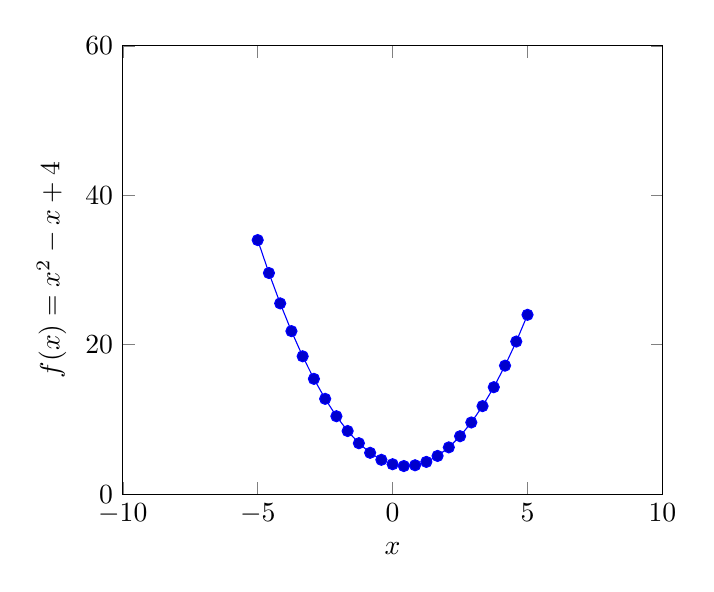
\begin{tikzpicture}
\begin{axis}[
    xlabel=$x$,
    xmin=-10,
    xmax=10,
    ymin=0,
    ymax=60,
    ylabel={$f(x) = x^2 - x +4$},
]
\addplot {x^2 - x +4};
\end{axis}
\end{tikzpicture}
\end{verbatim}
This will get rendered as:
\begin{center}
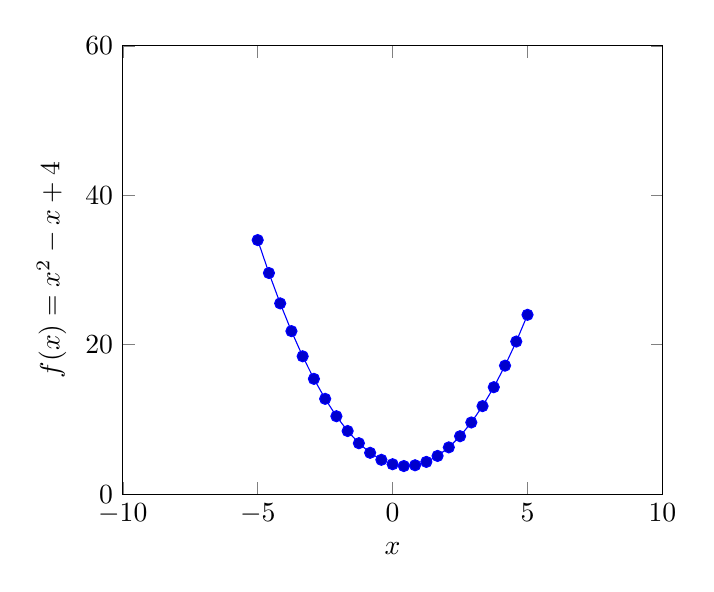
\begin{tikzpicture}
\begin{axis}[
    xlabel=$x$,
    xmin=-10,
    xmax=10,
    ymin=0,
    ymax=60,
    ylabel={$f(x) = x^2 - x +4$}
]
\addplot {x^2 - x +4};
\end{axis}
\end{tikzpicture}
\end{center}
Some other examples of "tikpicture" environment include:\\\\\\
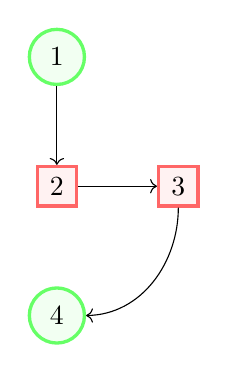
\begin{tikzpicture}[
    roundnode/.style={circle, draw=green!60, fill=green!5, very thick, minimum size=7mm},
    squarednode/.style={rectangle, draw=red!60, fill=red!5, very thick, minimum size=5mm},
]
\node[squarednode]      (maintopic)                              {2};
\node[roundnode]        (uppercircle)       [above=of maintopic] {1};
\node[squarednode]      (rightsquare)       [right=of maintopic] {3};
\node[roundnode]        (lowercircle)       [below=of maintopic] {4};
\draw[->] (uppercircle.south) -- (maintopic.north);
\draw[->] (maintopic.east) -- (rightsquare.west);
\draw[->] (rightsquare.south) .. controls +(down:7mm) and +(right:7mm) .. (lowercircle.east);
\end{tikzpicture}\\\\\\\\

\begin{tikzpicture}
\draw[blue, very thick] (0,0) rectangle (3,2);
\draw[orange, ultra thick] (4,0) -- (6,0) -- (5.7,2) -- cycle;
\end{tikzpicture}\\\\\\\\
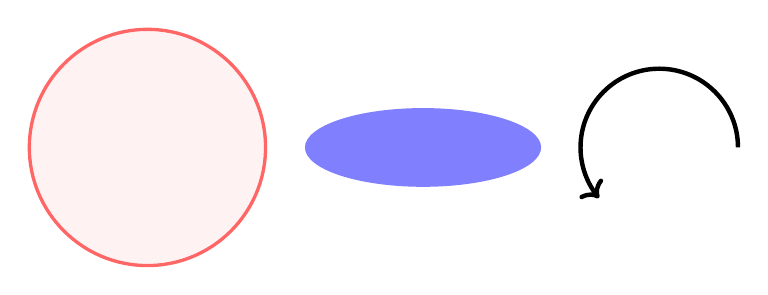
\begin{tikzpicture}
\filldraw[color=red!60, fill=red!5, very thick](-1,0) circle (1.5);
\fill[blue!50] (2.5,0) ellipse (1.5 and 0.5);
\draw[ultra thick, ->] (6.5,0) arc (0:220:1);
\end{tikzpicture}\\\\\\\\
\begin{tikzpicture}
\draw (-2,0) -- (2,0);
\filldraw [gray] (0,0) circle (2pt);
\draw (-2,-2) .. controls (0,0) .. (2,-2);
\draw (-2,2) .. controls (-1,0) and (1,0) .. (2,2);
\end{tikzpicture}\\\\\\\\
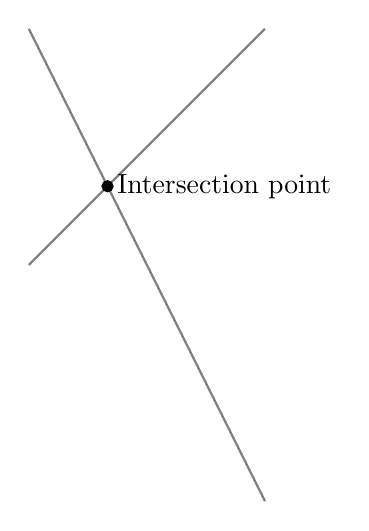
\begin{tikzpicture}
\draw[gray, thick] (-1,2) -- (2,-4);
\draw[gray, thick] (-1,-1) -- (2,2);
\filldraw[black] (0,0) circle (2pt) node[anchor=west] {Intersection point};
\end{tikzpicture}\\\\\\\\
If user adds "circuitikz" package it is possible to create circuit diagrams:\\\\
\begin{circuitikz}
    \draw (0,0)
    to[V,v=$U_q$] (0,2)
    to[short] (2,2)
    to[R=$R_1$] (2,0)
    to[short] (0,0);
    \draw (2,2)
    to[short] (4,2)
    to[L=$L_1$] (4,0)
    to[short] (2,0);
    \draw (4,2)
    to[short] (6,2)
    to[C=$C_1$] (6,0)
    to[short] (4,0);
 \end{circuitikz}
\section{Hyperlinks}
To embed clickable links in \LaTeX document import "hyperref" package and use one of following
commands:
\begin{verbatim}
My github page page:\href{https://github.com/mtracewicz}{github.com}\\
My github page page:\url{https://github.com/mtracewicz}\\
\end{verbatim}
Which will get rendered as:\\
My github page page:\href{https://github.com/mtracewicz}{github.com}\\
My github page page:\url{https://github.com/mtracewicz}\\
\bibliography{latex_introduction_bibliography}
\bibliographystyle{ieeetr}
\end{document}
